\chapter{Fisica della Tomografia ad Emissione di Positroni}
Il principio alla base delle tecniche PET consiste nella rilevazione simultanea di due raggi \textGamma generati da un evento di annichilazione \textit{elettrone-positrone}, generato da iniezione di un tracciante radioattivo in un soggetto. I positroni sono emessi dal nucleo di isotopi instabili e ricchi di protoni, durante il processo di decadimento radioattivo \cite{Bailey2014}. Infatti, questi isotopi acquisiscono la stabilità tramite un processo di decadimento che converte un protone in un neutrone, con la generazione di un positrone. Il positrone, chiamato anche \textit{antielettrone}, è l'antiparticella dell'elettrone. Infatti, esso ha la stessa massa e spin 1/2 dell'elettrone ma presenta una carica elettrica \textit{+e}. Più precisamente, il processo di decadimento che si verifica è di tipo \textit{beta plus} ($\beta^+$) in cui un protone legato ($p$) del nucleo dell'isotopo radioattivo si trasforma in un neutrone legato, un positrone ($e^+$) e un neutrino ($\nu_e$) \cite{Betaplus}. Il processo può essere riassunto dalla equazione:
\begin{equation}
	\text{p}\to \text{n} + e^+ + \nu_e.
\end{equation}
I \textit{tracer} radioattivi utilizzati nelle applicazione PET sono analoghi delle comuni molecole biologiche, come il glucosio, peptidi e proteine, in cui l'isotopo radioattivo viene utilizzato per sostituire un costituente della molecola. Un radiotracciante utilizzato per la tomografia ad emissione di positroni è il fluorodeossiglucosio (FDG), un analogo strutturale del glucosio, che viene captato dalle cellule ad alto utilizzo di glucosio, come quelle del cervello, del rene e quelle tumorali \cite{FDG}. Questa molecola è soggetta al decadimento, che porta la seguente reazione:
\begin{equation}
	^{18}_9\text{F}\to ^{18}_8\text{O} + e^+ + \nu_e.
\end{equation}
La molecola risultante diviene quindi una vera e propria molecola di \textit{glucosio-6-fosfato} normalmente metabolizzata dall'organismo. Per questa ragione, questa molecola può essere utilizzata per valutare la biodistribuzione del glucosio nell'organismo.

Una volta che il \textit{tracer} radioattivo è stato iniettato al paziente, raggiunge i tessuti target grazie al sistema circolatorio e dopo un certo tempo partecipa ai processi metabolici del soggetto. Durante il decadimento del tracciatore (circa 110 minuti per il $^{18}_9\text{F}$), i positroni generati collidono con gli elettroni degli atomi adiacenti tramite un processo di \textit{annichilazione positrone-elettrone} (\Fig\ref{fig:annihilation}). L'annichilazione genera due raggi gamma con un energia di \SI{511}{\kilo\electronvolt}, con un angolazione di circa \SI{180}{\degree}.
\begin{figure}[h]
	\centering
	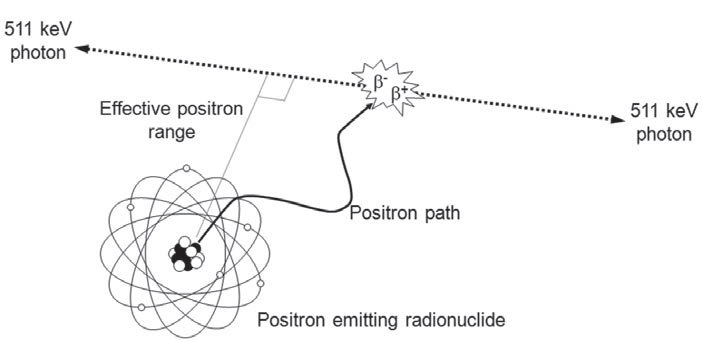
\includegraphics[width=0.8\linewidth]{./ImageFiles/annihilation}
	\caption{Processo di annichilazione \textit{positrone-elettrone} con generazione di due raggi gamma. Immagine tratta da Bailey D. et al\cite{Bailey2014}.}
	\label{fig:annihilation}
\end{figure}

\chapter{Sistema PET}
Nella figura \ref{fig:PET_imaging_system} è rappresentato un sistema di imaging PET. Per rilevare i raggi gamma derivanti dal processo di annichilazione \textit{elettrone-positrone}, viene utilizzato un rilevatore a scintillazione, composto da uno scintillatore e un fotorilevatore. 
\begin{figure}[h]
	\centering
	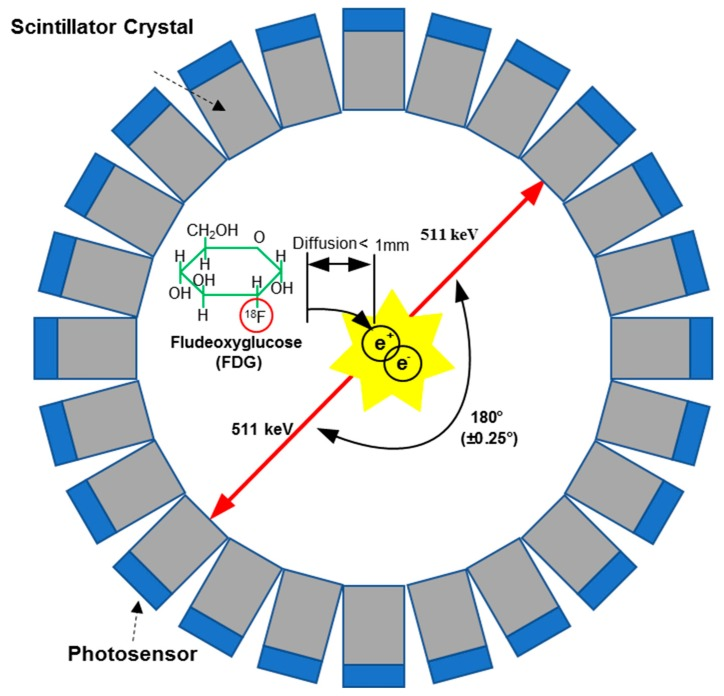
\includegraphics[width=0.5\linewidth]{./ImageFiles/PET_imaging_system}
	\caption{Principio di funzionamento di un sistema per tomografia ad emissione di positroni (PET). Un anello di sensori rilevano una coppia di raggi gamma con un'energia di \SI{511}{3\kilo\electronvolt} (frecce rosse) che derivano dalla annichilazione di un elettrone con un positrone emesso da un radiotracciante (FDG). Immagine tratta da Jiang W. et al \cite{Jiang2019}.}
	\label{fig:PET_imaging_system}
\end{figure}
\section{Scintillatori}
I cristalli scintillatori sono utilizzati per assorbire e convertire un raggio gamma ad alta energia in fotoni visibili a bassa energia, rilevati da opportuni sensori. Uno dei cristalli scintillatori più utilizzati è il \textit{Lutetium–(yttrium) oxyorthosilicate} (L(Y)SO) che garantisce una buona risoluzione di energia, alta luminosità in uscita e un tempo veloce di decadimento. Il processo di conversione di fotoni ad alta energia (raggi \textgamma) in luce visibile consiste in tre fasi \cite{RamseyDerek}:
\begin{itemize}
	\item un fotone incidente sul cristallo libera un elettrone (tramite effetto fotoelettrico o effetto Compton);
	\item quando l'elettrone attraversa il materiale, perde energia urtando ed eccitando altri elettroni;
	\item gli elettroni eccitati ritornano decadono al loro stato base, emettendo fotoni (sotto forma di impulsi di luce nel visibile).
\end{itemize}
Gli scintillatori utilizzati nei sistemi di acquisizione PET possono essere differenziati considerando quattro diverse proprietà \cite{Schmitz2013ThePO}:
\begin{itemize}
	\item stopping power;
	\item decay constant;
	\item energy resolution;
	\item light output.
\end{itemize}
Lo \textbf{stopping power} rappresenta l'inverso della distanza media percorsa dai fotoni prima di trasferire l'energia nel cristallo e dipende dalla densità e dal numero atomico effettivo del materiale. \`E preferibile che questo parametro sia alto (ossia poca distanza percorsa dai fotoni), in modo da avere più interazioni con i fotoni emessi dall'annichilazione \textit{elettrone-positrone}. La \textbf{decay constant}, invece, descrive la durata dell'impulso luminoso generato dal cristallo. \`E preferibile utilizzare cristalli con bassi valori di constante di decadimento in quanto permettono di rilevare un numero maggiore di impulsi a pari unità di tempo. Inoltre, è utile che il materiale abbia una buona risoluzione di energia (\textbf{energy resolution}), che descrive la capacità di distinguere raggi gamma con differenti energie. Infatti, nell'immagine \ref{fig:photo_peak} è mostrato lo spettro di distribuzione di energia, costruito misurando il numero di eventi rilevati con una certa ampiezza in funzione dell'energia depositata sul cristallo.
\begin{figure}[h]
	\centering
	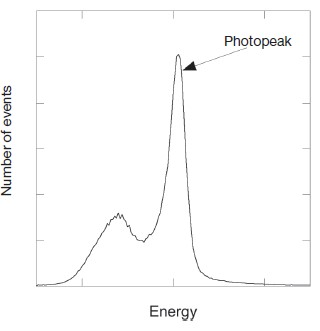
\includegraphics[width=0.4\linewidth]{./ImageFiles/Photo peak.jpg}
	\caption{Esempio di uno spettro di energia, definito come il numero di eventi misurati con una certa ampiezza in funzione della energia depositata sul cristallo. Immagine tratta da Bailey D et al. \cite{Bailey2014}.}
	\label{fig:photo_peak}
\end{figure}
Questa distribuzione è influenzata dalle caratteristiche del tracciatore radioattivo utilizzato e dal materiale con cui è realizzato il rilevatore. Tuttavia, è possibile sempre notare un picco marcato (denominato \textit{photopeak}), causato dall'assorbimento fotoelettrico, dove tutta l'energia del fotone è trasmessa all'elettrone. L'altra regione in cui l'energia si distribuisce è invece causata dall'effetto Compton, dove gli elettroni acquistano diversi valori di energia in base all'angolo di scattering. L'obiettivo delle tecniche di imaging della medicina nucleare è quello di riuscire a distinguere i raggi gamma che non hanno avuto interazioni con altri tessuti, che ne hanno provocato una deviazione. I fotoni di interesse sono proprio quelli i cui raggi \textgamma hanno energia pari al \textit{photopeak} e che, non essendo stati soggetti a fenomeni di scattering, permettono di risalire in modo accurato alla posizione del radionuclide. Tipicamente, il \textit{photopeak} si presenta in un valore di energie nell'intervallo \numrange[range-phrase=--]{440}{650}\,\unit{\kilo\electronvolt}. Infine, il parametro \textbf{light output} definisce il numero di fotoni emessi durante la scintillazione prodotti da ogni fotone incidente. Il valore di questo parametro dovrebbe essere il più alto possibile per garantire la massima risoluzione spaziale e di energia.

\noindent
Il confronto tra alcune caratteristiche di diversi scintillatori utilizzati negli scanner PET sono riportate nella tabella \ref{tab:scintillator_properties}.

\begin{table}[tbh]
	\centering
	\begin{tabular}{l|ccc}
		\hline
		\textbf{Cristallo} & NaI & BGO & LSO (LYSO) \\ \hline
		\textbf{Stopping power} ($\unit{\centi\meter}^{-1}$) & 0.34 & 0.92 & 0.87  \\ \hline
		\textbf{Decay constant} (\unit{\nano\second}) & 230 & 300 & 40 \\ \hline
		\textbf{Light output} (\%NaI:TI) & 100 & 15 & 75 \\ \hline
	\end{tabular}
	\caption{Proprietà dei materiali scinitallori utilizzati negli scanner PET. Dati tratti da \cite{RamseyDerek}.}
	\label{tab:scintillator_properties}
\end{table}

\section{Fotorilevatori}
Per convertire il segnale luminoso in segnale elettrico si utilizzano dei fotorilevatori, come ad esempio i \textit{Photomultiplier Tubes} (PMTs), Avalanche Photodiodes (ADPs) e i Silicon Photomultipliers (SiPMs). Si creano quindi dei moduli (\Fig\ref{fig:photodetectors}) costituiti da uno scintillatore montato su un fotorilevatore.
\begin{figure}[tbh]
	\centering
	a)
	\begin{minipage}{.45\textwidth}
		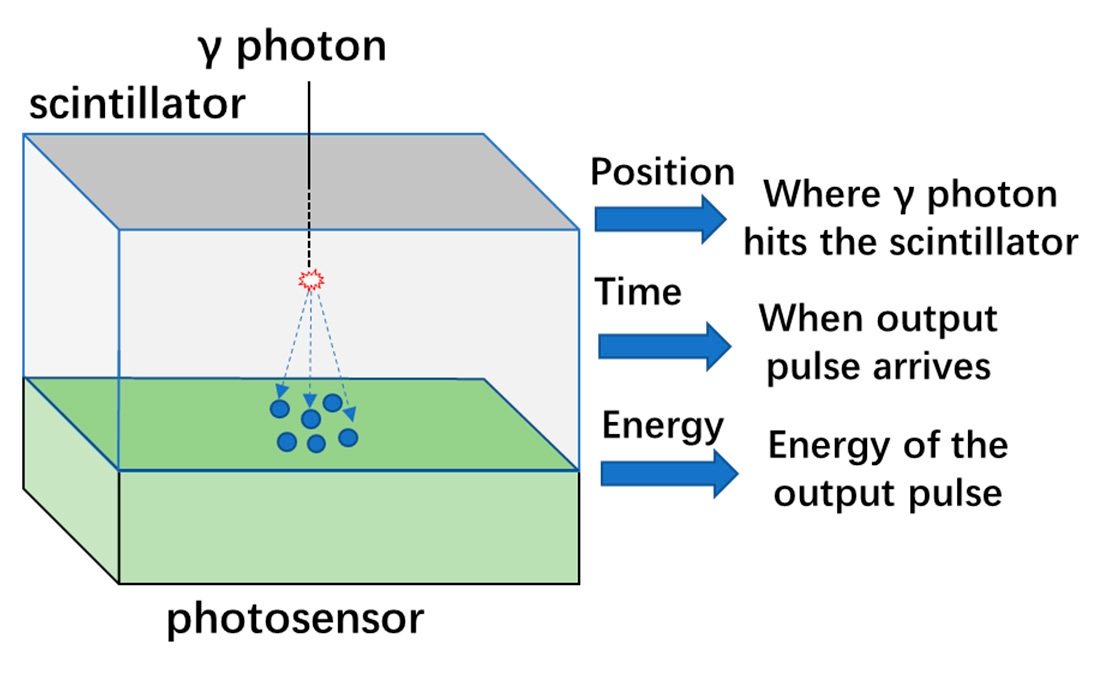
\includegraphics[width=\linewidth]{./ImageFiles/PET_detectors.jpg}
	\end{minipage}
	b)
	\begin{minipage}{.45\textwidth}
		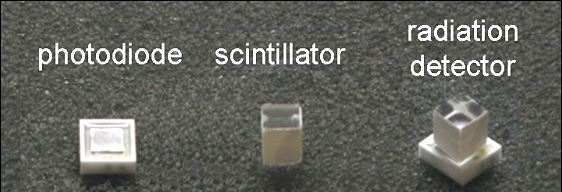
\includegraphics[width=\linewidth]{./ImageFiles/PET_detectors_real.jpg}
	\end{minipage}
	\caption{Struttura di un sensore PET. Immagini tratte da \cite{Jiang2019} e da \cite{Spanoudaki2010}.}
	\label{fig:photodetectors}
\end{figure}
Questi \textit{detectors} modulari sono poi uniti per formare un anello al centro del quale rilevare i raggi gamma (\Fig\ref{fig:PET_imaging_system}). I rilevatori utilizzati per la PET devono permettere di ricavare tre tipi di informazioni:
\begin{itemize}
	\item la posizione di dove il raggio gamma impatta lo scintillatore;
	\item il tempo in cui si verifica l'impulso luminoso;
	\item l'energia dell'impulso luminoso generato.
\end{itemize}
Di seguito si analizzano alcuni fotorivelatori utilizzati nei sistemi PET.
\subsection{Photomultiplier Tubes}
Nella figura \ref{fig:ptm} è mostrato lo schema della struttura di un fotomoltiplicatore PMT (\textit{Photomultiplier Tube}).
\begin{figure}[tbh]
	\centering
	a)
	\begin{minipage}{.70\textwidth}
		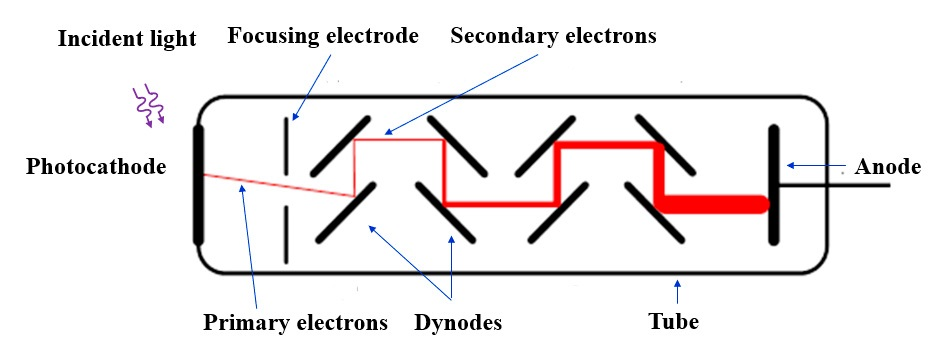
\includegraphics[width=\linewidth]{./ImageFiles/ptm.jpg}
	\end{minipage}

	b)
	\begin{minipage}{.70\textwidth}
		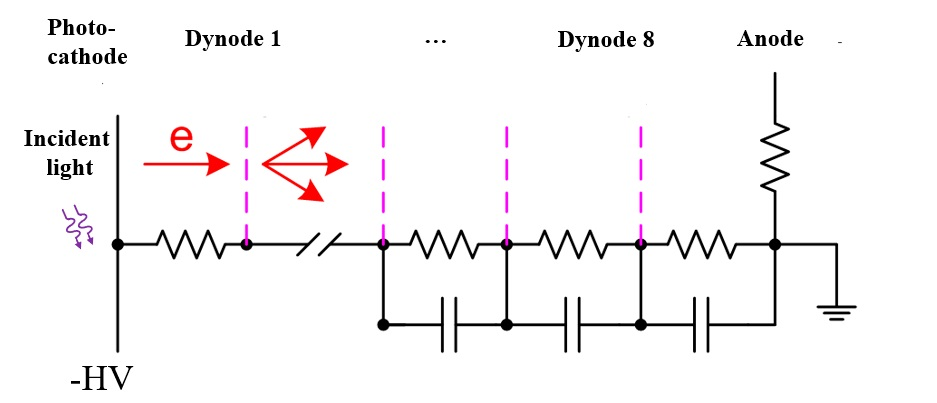
\includegraphics[width=\linewidth]{./ImageFiles/ptm_schema.jpg}
	\end{minipage}
	\caption{Principio di funzionamento di un \textit{photomultiplier tube} (PTM): a) struttura semplificata; b) schema semplificato del circuito di polarizzazione ad alta tensione. Immagine tratta da Jiang et al. \cite{Jiang2019}.}
	\label{fig:ptm}
\end{figure}
Esso è composto da un \textit{fotocatodo}, una serie di elettrodi chiamati \textit{dinodi} e un \textit{anodo}, inseriti in un tubo di vetro al cui interno è stato praticato il vuoto. Ai differenti dinodo è applicata una tensione crescente che permette di aumentare progressivamente il campo elettrico all'interno del tubo. I fotoni incidenti sul fotocatodo (ricoperto da un materiale che favorisce l'effetto fotoelettrico) generano degli elettroni (denominati \textit{fotoelettroni}) che vengono focalizzati da un elettrodo verso il primo dinodo. A causa del forte campo elettrico generato dalla differenza di potenziale tra il primo dinodo e il fotocadoto, gli elettroni primari aumentano la propria energia cinetica. Quando un elettrone fotogenerato colpisce il primo dinodo provoca l'emissione secondaria di diversi elettroni con minore energia. La struttura è realizzata in modo che ciascun elettrone secondario venga accelerato verso il dinodo successivo e provochi quindi l'emissione di ulteriori elettroni secondari. Si instaura così un fenomeno a cascata per cui un singolo elettrone fotogenerato genera un numero di elettroni pari a 
\begin{equation}
	G = f^n,
\end{equation}
dove $f$ è il fattore di emissione di elettroni secondari di ogni dinodo e n è il numero di dinodi. Valori tipici delle tensioni di alimentazioni sono  compresi nell'intervallo di \numrange[range-phrase=--]{1000}{2000}\,\unit{\kilo\volt} e il guadagno $G$ raggiunto è di circa di $G=10^6$. Per determinare la posizione dell'interazione \textit{fotone-cristallo scintillatore}, è possibile utilizzare una struttura definita a \textit{block detector} (\Fig\ref{fig:block_detector}).
\begin{figure}[tbh]
	\centering
	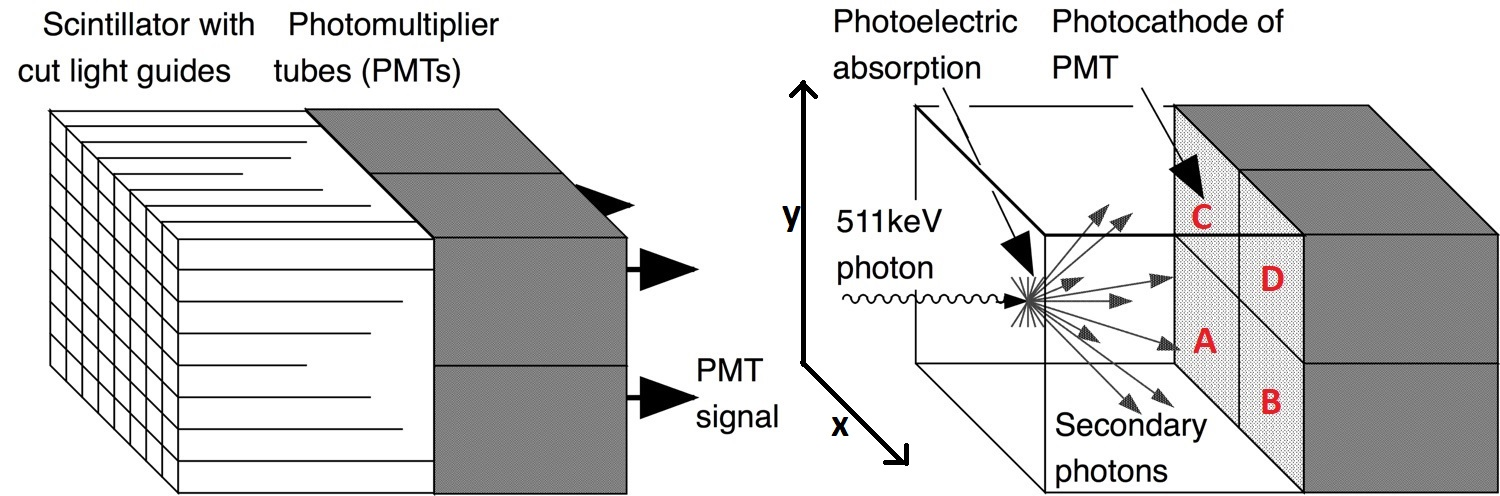
\includegraphics[width=0.8\linewidth]{./ImageFiles/block_detector.jpg}
	\caption{Schema della struttura di un \textit{block detector} con piccoli cristalli scintillatori raggruppati in blocchi accoppiati a quattro PMT. Immagine tratta da Schmitz et al. \cite{Schmitz2013ThePO}}. 
	\label{fig:block_detector}
\end{figure}
Viene ricavato da un cristallo una matrice di blocchi scitillatori (di dimensioni di qualche millimetro), suddivisi da un materiale riflettente. Gli impulsi luminosi emessi vengono letti da 4 differenti PMT (\Fig\ref{fig:block_detector_cube}).
\begin{figure}[tbh]
	\centering
	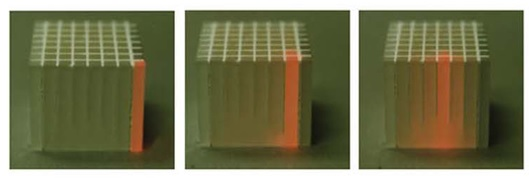
\includegraphics[width=0.6\linewidth]{./ImageFiles/block_detector_lightoncube.jpg}
	\caption{Distribuzione della luce in un cristallo scintillatore suddiviso in una matrice di cristalli. Immagine tratta da Terry Jones and David Townsend \cite{Jones2017}}. 
	\label{fig:block_detector_cube}
\end{figure}
Confrontando le intensità rilevate dai quattro PMT con dei valori pre-calcolati, è possibile ricavare la posizione del fotone incidente sul piano tramite le seguenti equazioni \cite{RamseyDerek} (logica di Anger):
\begin{equation}
	\begin{split}
		R_X&=\frac{A+B}{A+B+C+D} \\
		R_Y&=\frac{A+C}{A+B+C+D}, \\
	\end{split}
\end{equation}
dove $A,B,C,D$ rappresentano la frazione di luce misurata dai quattro PMT.

Idealmente, se nessun fotone viene assorbito dal fotocatodo (ossia se il sensore viene tenuto al buio), non ci sarà nessun segnale all'anodo del PMT. Tuttavia, statisticamente c'è una probabilità non nulla che degli elettroni vengano emessi dal fotocadoto e dai dinodi per effetto termoionico, generando un impulso. Ciò determina il parametro di\textit{dark count rate} (DCR) del PMT (tipicamente pari a 10 impulsi al secondo). \todo{inserire pag 8 sesnor for positron TTR e TTs}
Un altro parametro di interesse per descrivere un PMT è la \textit{Photon detection efficiency} (PDE) che descrive la probabilità di emissione di un elettrone fotogenerato per ogni fotone incidente, che dipende dalla \textit{quantum efficiency} (QE) del materiale che ricopre il fotocatodo e dalla \textit{collection efficiency} (CE), ossia il rapporto tra il numero di elettroni che giungono al primo dinodo e quelli generati dal fotocatodo \cite{Hai2018}. La QE di un PMT è tipicamente pari al \SI{25}{\percent}, ma la PDE assume un valore minore a causa della CE, dal momento che non tutti gli elettroni fotogenerati generano un impulso luminoso.

Sebbene i PMT abbiano un alto guadagno, alta risoluzione nel tempo, basso \textit{noise} e una QE accettabile, presentano alcuni svantaggi. Infatti, sono molto fragili e sensibili a vibrazioni meccani e disturbi elettromagnetici e necessitano di alte tensioni di alimentazione. Per questo motivo sono state sviluppate soluzioni a stato solido come gli ADP e i SiPM.

\newpage
\subsection{Avalanche Photodiodes}
Gli \textit{avalanche photodiodes} (APDs) sono diodi che strutturalmente sono simili ai p-n e p-i-n fotodiodi ma presentano un meccanismo di guadagno determinato da un eventi "a valanga". Essi sono fortemente polarizzati inversamente, generando un forte campo magnetico nella zona di svuotamento. In questo modo, quando un elettrone viene generato da un fotone incidente (effetto fotoelettrico) nella zona di svuotamento subisce una accelerazione tale che, all'impatto con gli atomi del reticolo del substrato, genera una coppia elettrone-lacuna (\Fig\ref{fig:adp}).  

\begin{figure}[tbh]
	\centering
	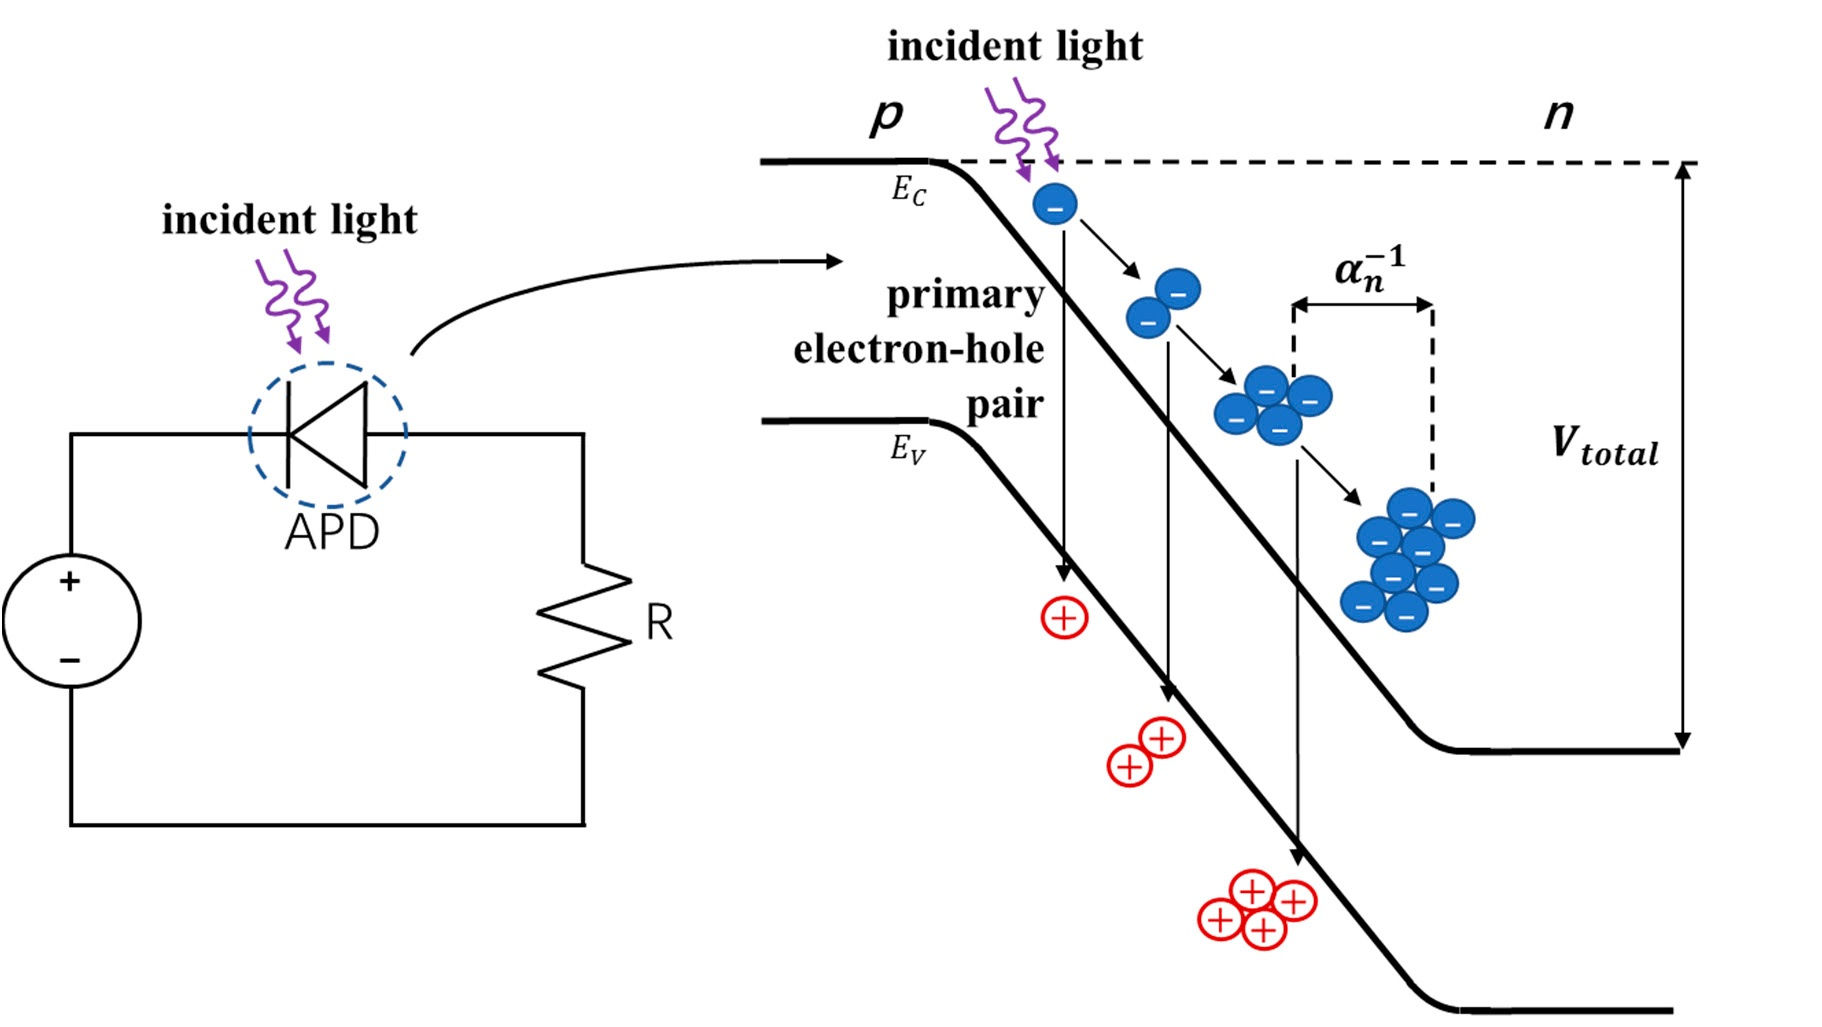
\includegraphics[width=0.8\linewidth]{./ImageFiles/ADP.jpg}
	\caption{Effetto a valanga in un ADP. $\alpha_n^{-1}$ è la distanza media tra ogni evento di moltiplicazione e $V_{TOT}$ è la tensione di polarizzazione (sommata al potenziale di built-in). Immagine tratta da Wei Jiang et al. \cite{Jiang2019}.} 
	\label{fig:adp}
\end{figure}


\subsection{Silicon Photomultipliers}

\subsection{CZT}


\todo{tabella con proprietà dei fororilavatori da Spanoudaki, }
\section{Principio di funzionamento}

\section{TOF PET}